\documentclass{article}
\usepackage[utf8]{inputenc}
\usepackage{hyperref}
\usepackage{geometry}
\geometry{a4paper, margin=1in}
\usepackage{lipsum} % For dummy text
\usepackage{graphicx} % Add this line to include the graphicx package
\hypersetup{
    colorlinks=true,
    linkcolor=black,
    urlcolor=blue,
    }


\title{Sales Dashboard Documentation}
\author{Ludovic Lafon}
\date{\today}

\begin{document}

\maketitle
\tableofcontents
\clearpage % Add a new page after the table of contents

\section{Introduction}

\subsection{Purpose of the Document}
This document provides comprehensive documentation of the sales dashboards developed using Tableau. It is intended for sales managers, business executives, and analysts who will be using these dashboards to monitor and analyze sales performance.

\subsection{Overview of the Sales Dashboard}
The sales dashboards include the Homepage Dashboard, Revenue Dashboard, Product Performance Dashboard, Sales Team Dashboard, and Pipeline Analysis Dashboard. Each dashboard is designed to provide insights into different aspects of the sales process, from overall revenue to individual sales agent performance.

\subsection{Importance of Sales Dashboards}
Sales dashboards are crucial for making data-driven decisions. They allow for real-time tracking of key performance indicators (KPIs), identification of trends and patterns, and optimization of sales strategies.

\subsection{Data Sources}
The dashboards integrate data from a fictional company's CRM system, which is available on Kaggle. The dataset includes information about customer interactions, sales activities, and opportunities. The data was cleaned, transformed, and integrated using Pandas in a separate Python notebook file, which is  \href{[https://github.com/LAlto96/sales-analytics-dashboard]}{available on GitHub}.

\subsubsection{About the Dataset}
\textbf{Description:}
This dataset contains information about customer interactions, sales activities, and opportunities from a fictional company's CRM (Customer Relationship Management) system. The dataset is designed to help data scientists and analysts understand the sales process, identify trends and patterns, and build predictive models to improve sales performance.
\\
\\
\noindent \textbf{Features:}
\begin{itemize}
    \item Customer information (demographics, firmographics, etc.)
    \item Sales activities
    \item Opportunity data (deal size, stage, probability, etc.)
    \item Product/service information
    \item Sales team and performance metrics
    \item Time-series data (daily/weekly/monthly sales, etc.)
\end{itemize}

\noindent \textbf{Use Cases:}
\begin{itemize}
    \item Predicting won/lost opportunities
    \item Forecasting deal size
    \item Identifying key drivers of sales performance
    \item Optimizing sales team performance
    \item Analyzing customer behavior and preferences
\end{itemize}

This dataset is perfect for data scientists, analysts, and students looking to practice their skills in:
\begin{itemize}
    \item Predictive modeling
    \item Data visualization
    \item Sales analytics
    \item Customer relationship management
\end{itemize}

Get started: Download the dataset and start exploring!

\subsection{Dashboard Specifications}

\subsubsection{Dashboard Requirements}

\noindent \textbf{Key Metrics and KPIs:}
\begin{itemize}
    \item Total Revenue
    \item Deal Conversion Rate
    \item Average Deal Size
    \item Sales by Product
    \item Top Performing Sales Agents
    \item Sales Pipeline Status
    \item Win Rate
    \item Average Sales Cycle Length
    \item Revenue by Sector
    \item Customer Acquisition Cost (CAC)
    \item Customer Lifetime Value (CLV)
    \item Lead Response Time
    \item Deal Stage Duration
    \item Regional Sales Performance
    \item Sales Forecast Accuracy
\end{itemize}

\noindent \textbf{User Stories:}
\begin{itemize}
    \item As a Sales Manager, I want to see the total revenue generated by the sales team to assess overall performance.
    \item As a Business Executive, I want to analyze the deal conversion rate to understand the efficiency of the sales process.
    \item As a Potential Client, I want to see the top-performing products to understand the company’s product strengths.
    \item As a Regional Manager, I want to monitor the performance of sales agents in my region to provide targeted support and training.
    \item As a CEO, I want to see the win rate to understand the overall success rate of our sales efforts.
    \item As a Sales Director, I want to analyze the average sales cycle length to identify bottlenecks in the sales process.
    \item As a Marketing Manager, I want to understand the customer acquisition cost to evaluate the efficiency of our marketing campaigns.
    \item As a Financial Analyst, I want to calculate the customer lifetime value to help with financial forecasting and budgeting.
    \item As a Sales Trainer, I want to review the lead response time to improve training programs for quicker lead engagement.
    \item As a Regional Manager, I want to compare sales performance across different regions to identify high and low performing areas.
    \item As an Operations Manager, I want to track deal stage duration to optimize the sales process and reduce delays.
    \item As a Sales Analyst, I want to assess sales forecast accuracy to improve our sales planning and predictions.
    \item As a Business Development Manager, I want to see revenue by sector to target high-potential industries for growth.
\end{itemize}


\subsection{Structure of the Document}
This document is organized into several sections, each covering a specific dashboard:
\begin{itemize}
    \item Homepage Dashboard: Overview and key metrics.
    \item Revenue Dashboard: Detailed revenue metrics and trends.
    \item Product Performance Dashboard: Insights into product sales and performance.
    \item Sales Team Dashboard: Analysis of sales agent performance.
    \item Pipeline Analysis Dashboard: Visualization of the sales pipeline stages and performance.
\end{itemize}
\clearpage

\section{Homepage Dashboard}
% Homepage Dashboard content goes here.
\begin{figure}[h!]
    \centering
    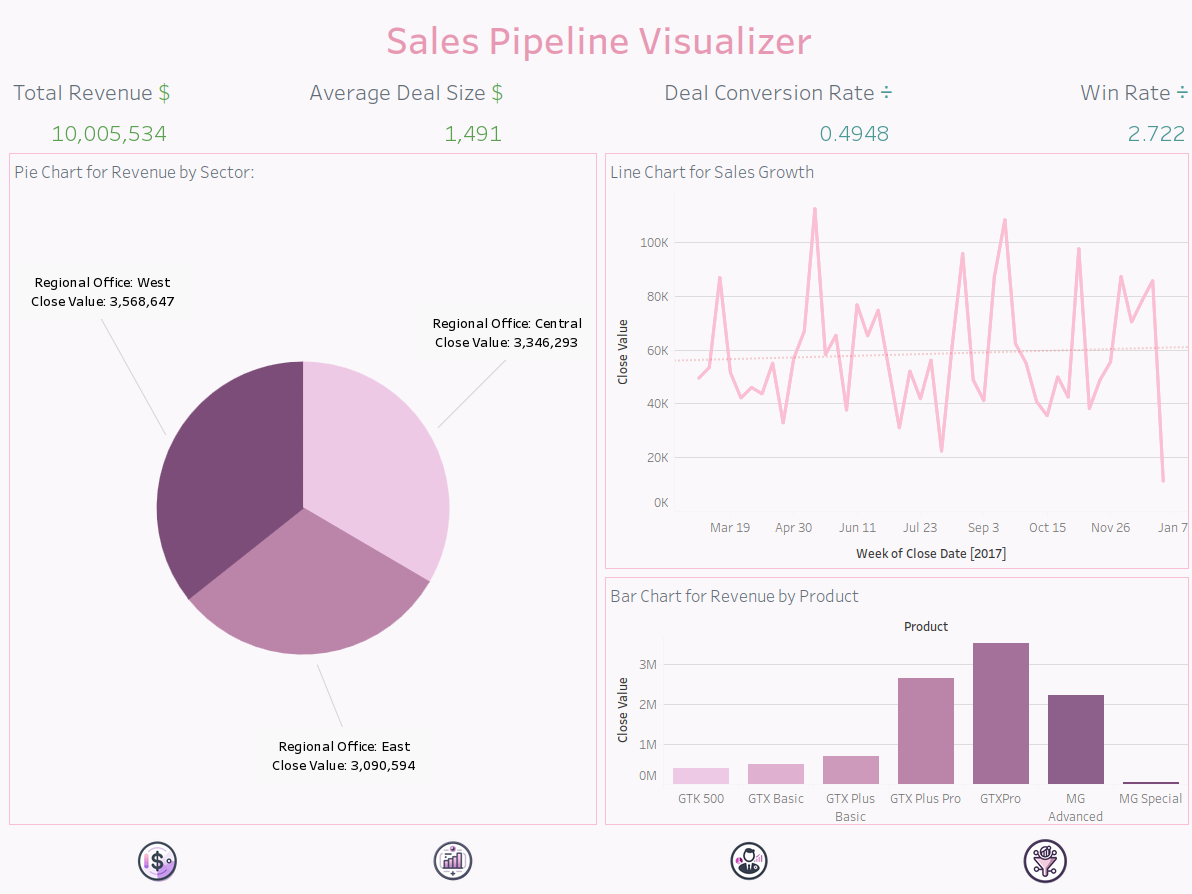
\includegraphics[width=0.8\textwidth]{resources/swappy-20240527_141415.png}
    \caption{Homepage}
\end{figure}

The Homepage provides a comprehensive overview of the company's revenue performance. It includes key metrics and visualizations that help in understanding the revenue trends, distribution across different regions, and performance of various products.

\subsection{Key Metrics}
The key metrics displayed in the Homepage are:
\begin{itemize}
    \item \textbf{Total Revenue:} This metric shows the total revenue generated over a specified period.
    \item \textbf{Average Deal Size:} This metric indicates the average revenue per deal.
    \item \textbf{Deal Conversion Rate:} This metric represents the percentage of deals that were successfully closed.
    \item \textbf{Win Rate:} This metric shows the percentage of deals won out of the total deals engaged.
\end{itemize}

\subsection{Visualizations}
The Homepage includes the following visualizations:
\begin{itemize}
    \item{Pie Chart for Revenue by Sector:}
    \item{Line Chart for Sales Growth:}
    \item{Bar Chart for Revenue by Product:}
\end{itemize}
Both the bar chart and the pie chart can act as filters for the entire Homepage. Users can click on a specific segment of the pie chart or bar to filter the data across all visualizations on the Homepage, allowing for a more interactive and detailed analysis.
\begin{figure}[h!]
    \centering
    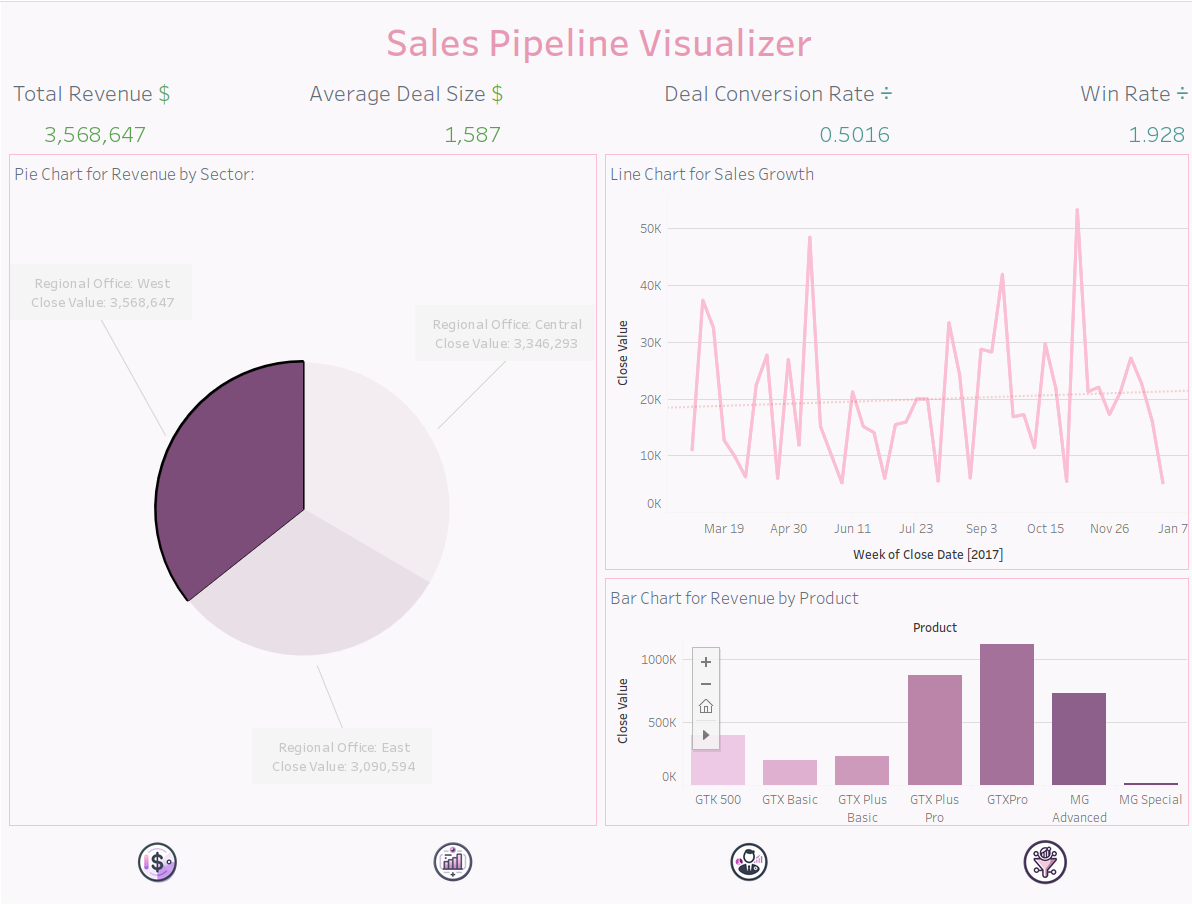
\includegraphics[width=0.8\textwidth]{resources/swappy-20240527_141440.png}
    \caption{\scriptsize{Pie Chart applying a filter on Regional West office.}}
\end{figure}
\begin{figure}[h!]
    \centering
    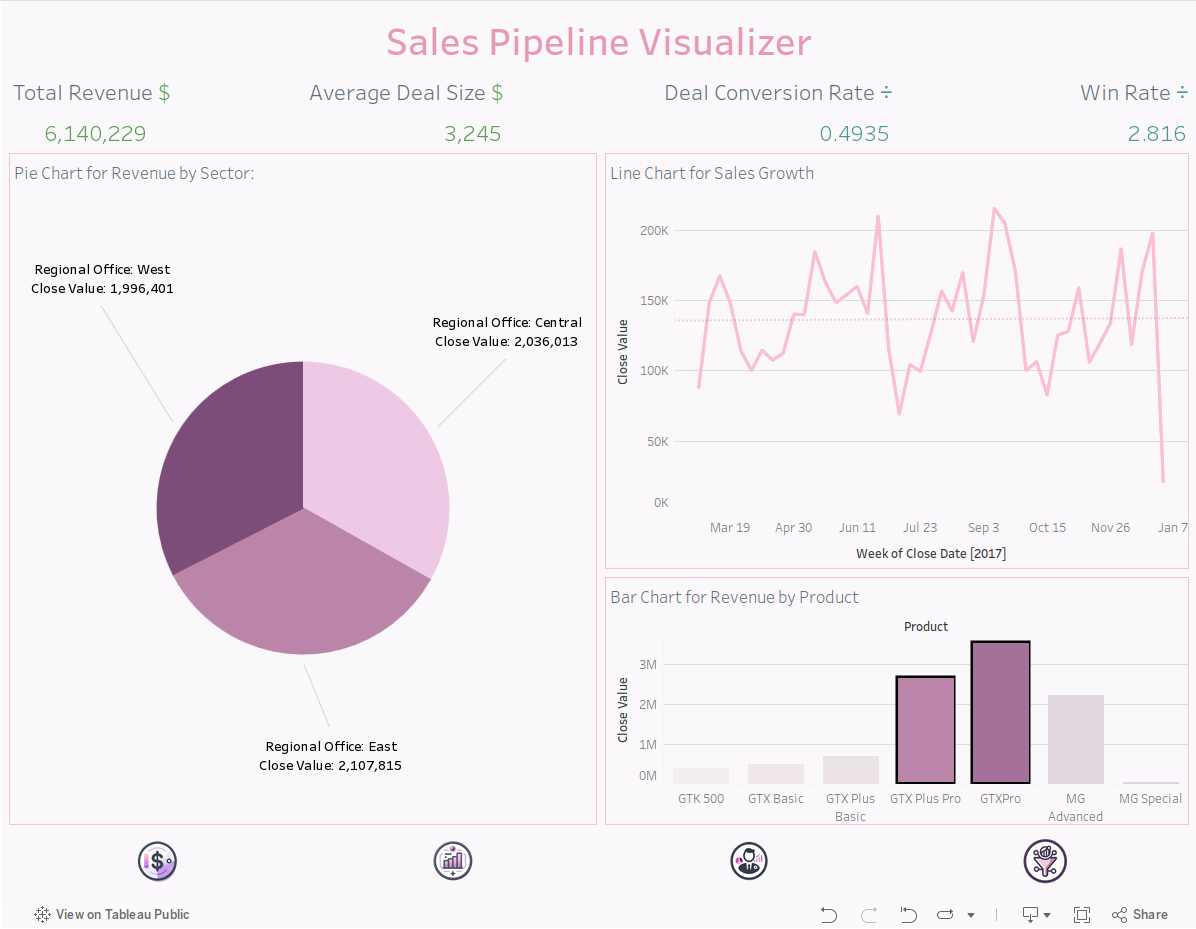
\includegraphics[width=0.8\textwidth]{resources/swappy-20240527_141503.png}
    \caption{\scriptsize{Bar Chart applying a filter on GTXPro and GTXPlus Pro products.}}
\end{figure}

\subsection{Interactive Navigation}
The dashboard also includes interactive navigation icons at the bottom, which allow users to switch between different views and dashboards easily.

\begin{figure}[h!]
    \centering
    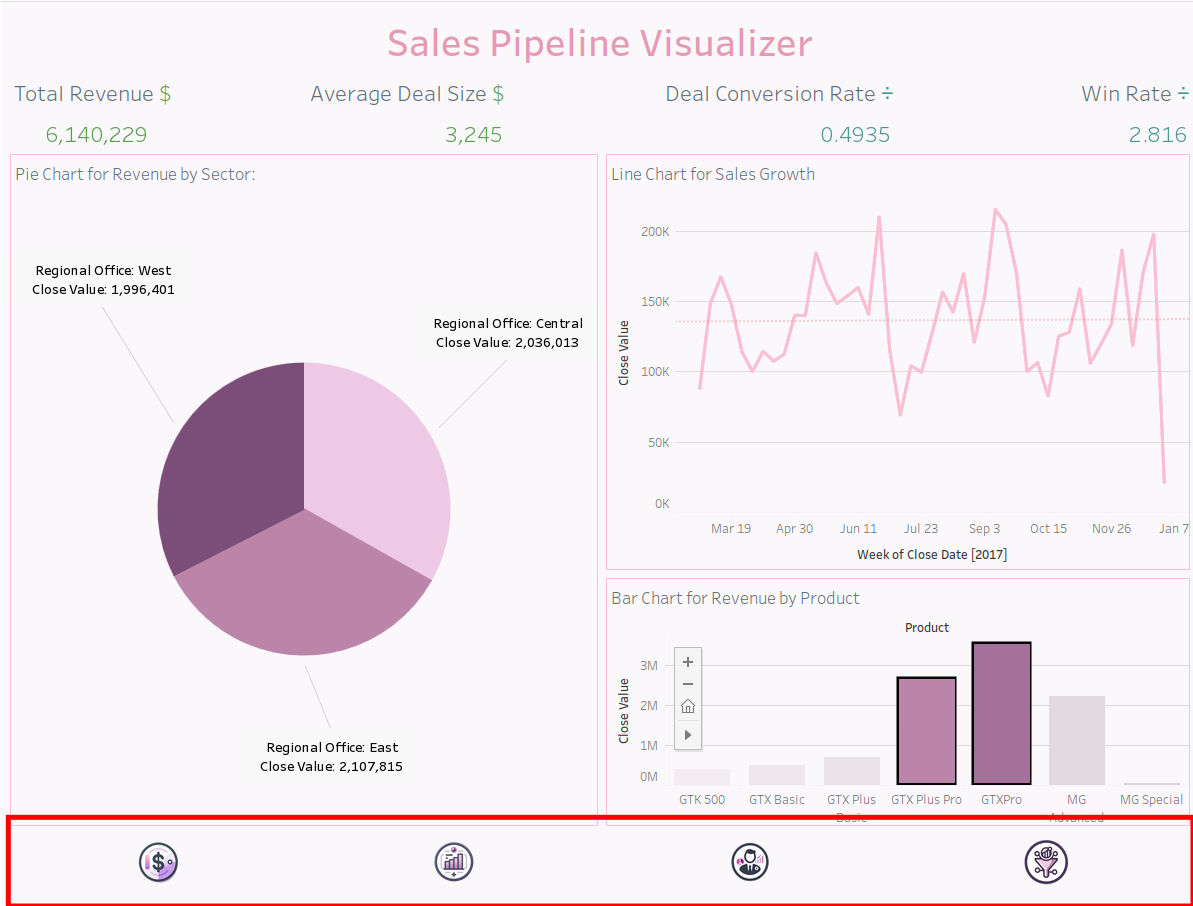
\includegraphics[width=0.8\textwidth]{resources/swappy-20240527_141526.png}
    \caption{Interactive Navigation Icons}
    \label{fig:navigation_icons}
\end{figure}

\clearpage

\section{Revenue Dashboard}
% Revenue Dashboard content goes here.
\begin{figure}[h!]
    \centering
    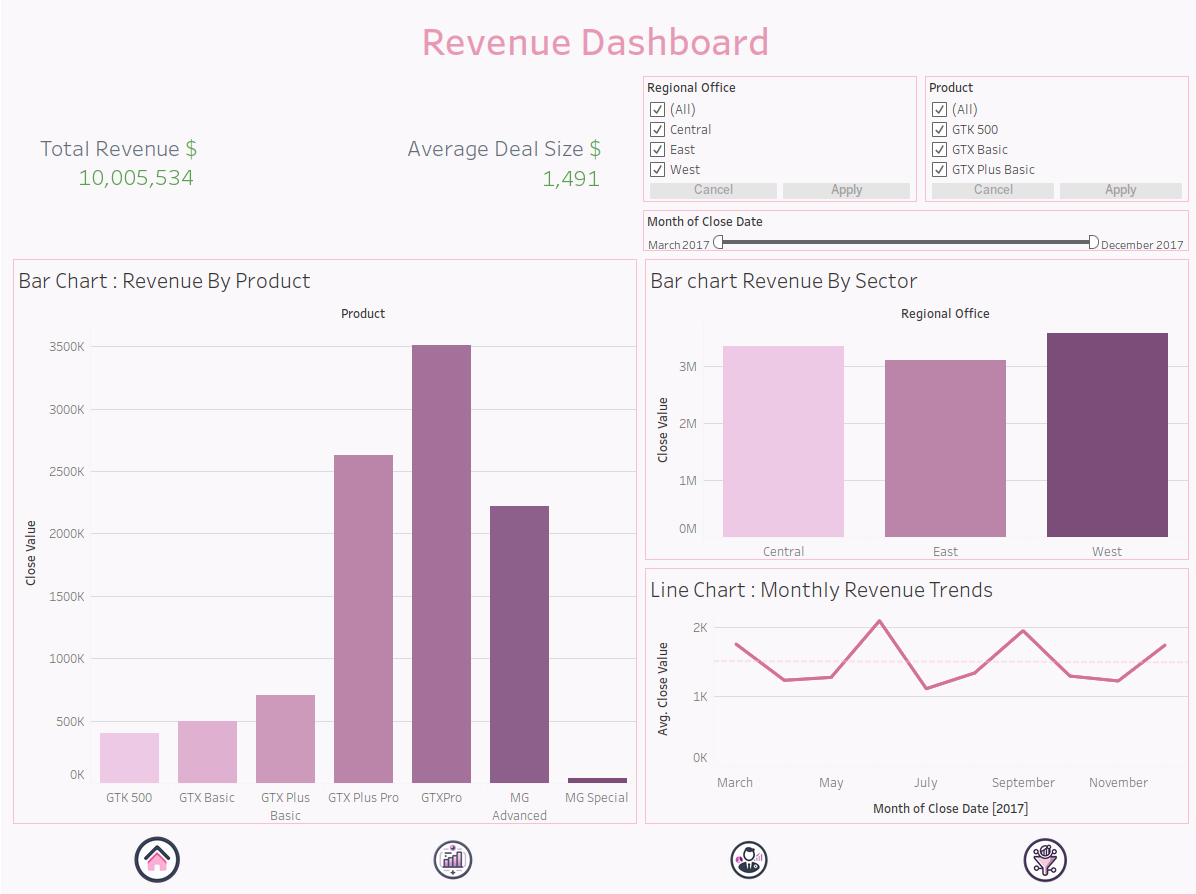
\includegraphics[width=0.8\textwidth]{resources/swappy-20240527_152429.png}
    \caption{Overview of the Revenue Dashboard}
    \label{fig:revenue_dashboard_overview}
\end{figure}
The Revenue Dashboard provides a comprehensive overview of the company's revenue performance. It includes key metrics and visualizations that help in understanding the revenue trends, distribution across different regions, and performance of various products.

\subsection{Key Metrics}
The key metrics displayed in the Revenue Dashboard are:
\begin{itemize}
    \item \textbf{Total Revenue:} This metric shows the total revenue generated over a specified period.
    \item \textbf{Average Deal Size:} This metric indicates the average revenue per deal.
    \item \textbf{Deal Conversion Rate:} This metric represents the percentage of deals that were successfully closed.
    \item \textbf{Win Rate:} This metric shows the percentage of deals won out of the total deals engaged.
\end{itemize}

\subsection{Visualizations}
The Revenue Dashboard includes the following visualizations:
\begin{itemize}
    \item \textbf{Bar Chart for Revenue by Product:} This bar chart displays the revenue generated by each product.
    \item \textbf{Bar Chart for Revenue by Sector:} This bar chart shows the revenue distribution across different sectors.
    \item \textbf{Line Chart for Monthly Revenue Trends:} This line chart illustrates the revenue trends on a monthly basis.
\end{itemize}


\subsection{Interactive Navigation}
Both the bar chart and the pie chart can act as filters for the entire Revenue Dashboard. Users can click on a specific segment of the pie chart or bar to filter the data across all visualizations on the Revenue Dashboard, allowing for a more interactive and detailed analysis.There is also a {Date Range Filter}

\begin{figure}[h!]
    \centering
    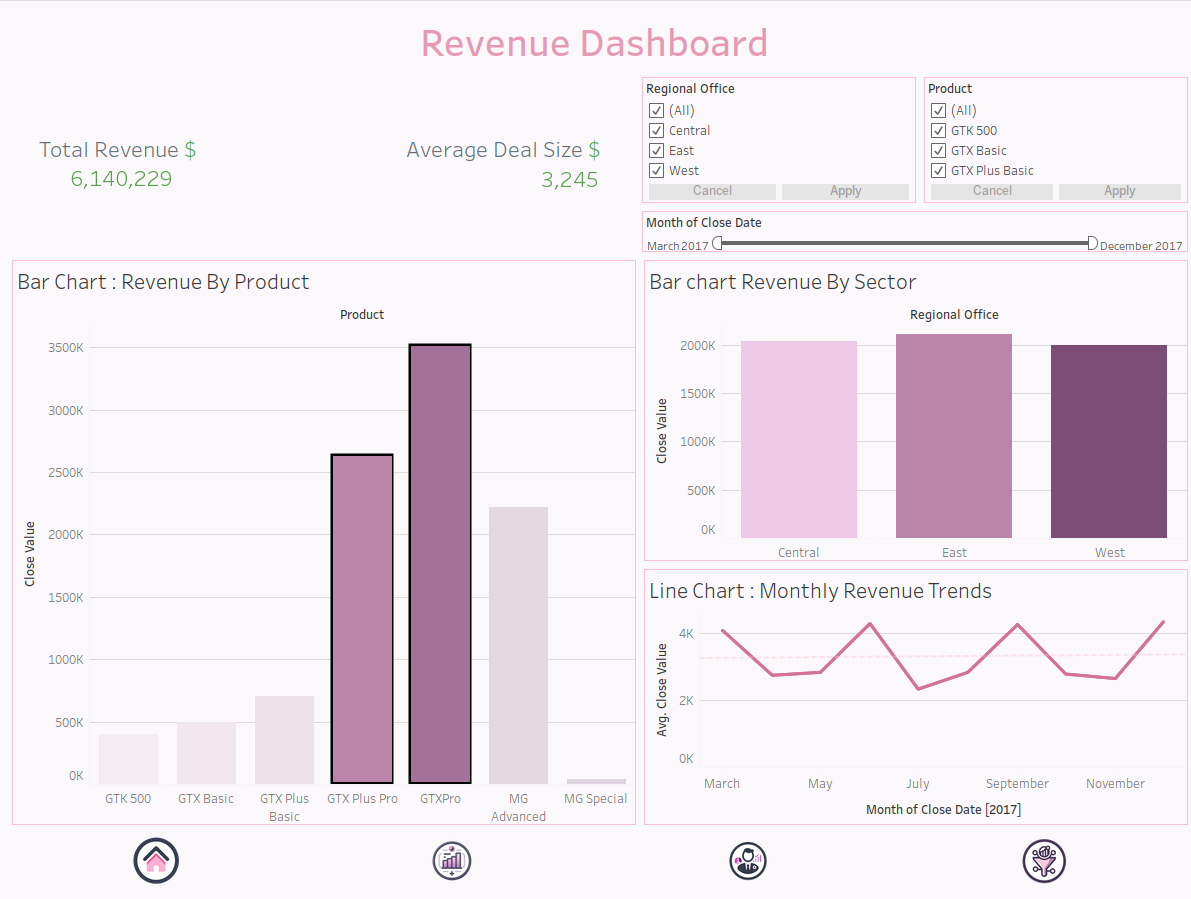
\includegraphics[width=0.8\textwidth]{resources/swappy-20240527_152442.png}
    \caption{Bar Chart for Revenue by Sector}
    \label{fig:revenue_by_sector_bar_chart}
\end{figure}

\begin{figure}[h!]
    \centering
    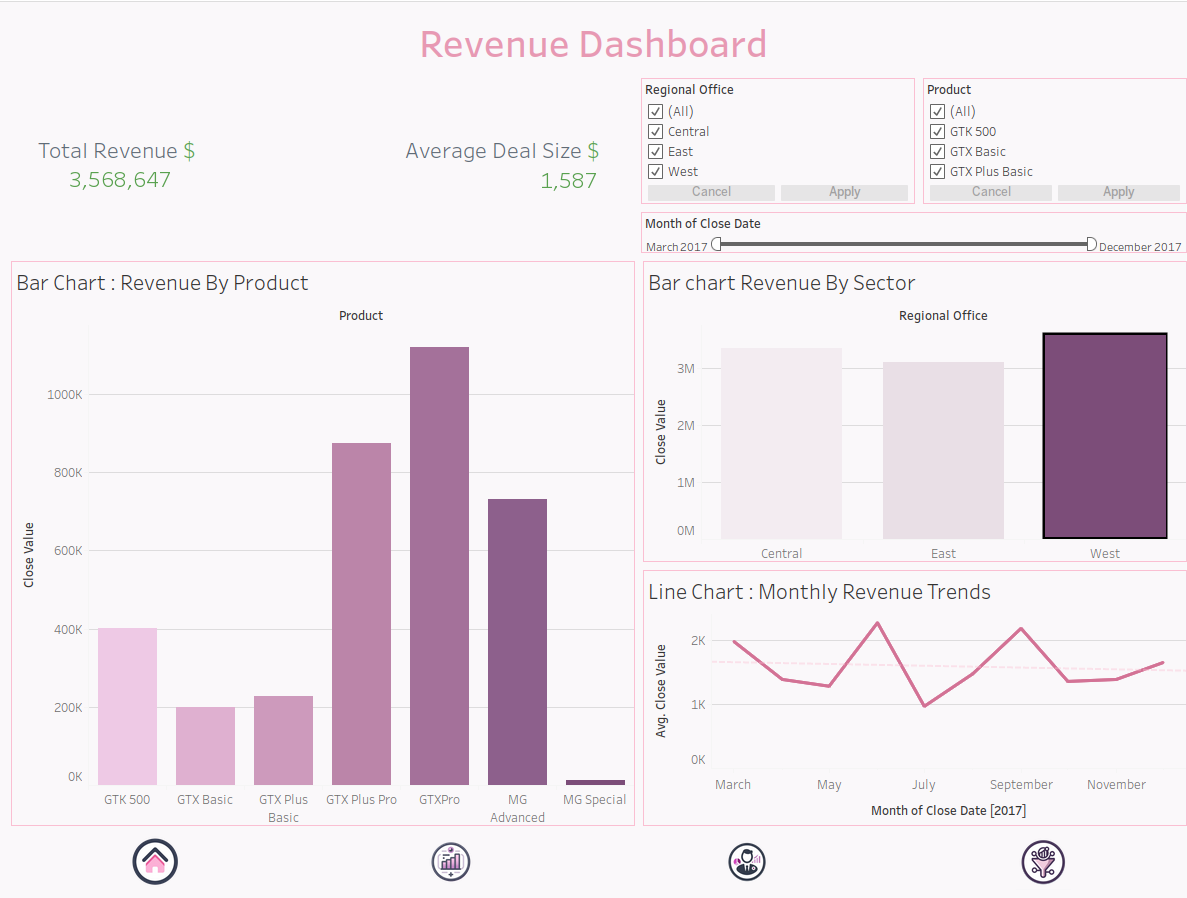
\includegraphics[width=0.8\textwidth]{resources/swappy-20240527_152507.png}
    \caption{Line Chart for Monthly Revenue Trends}
    \label{fig:monthly_revenue_trends_line_chart}
\end{figure}

\begin{figure}[h!]
    \centering
    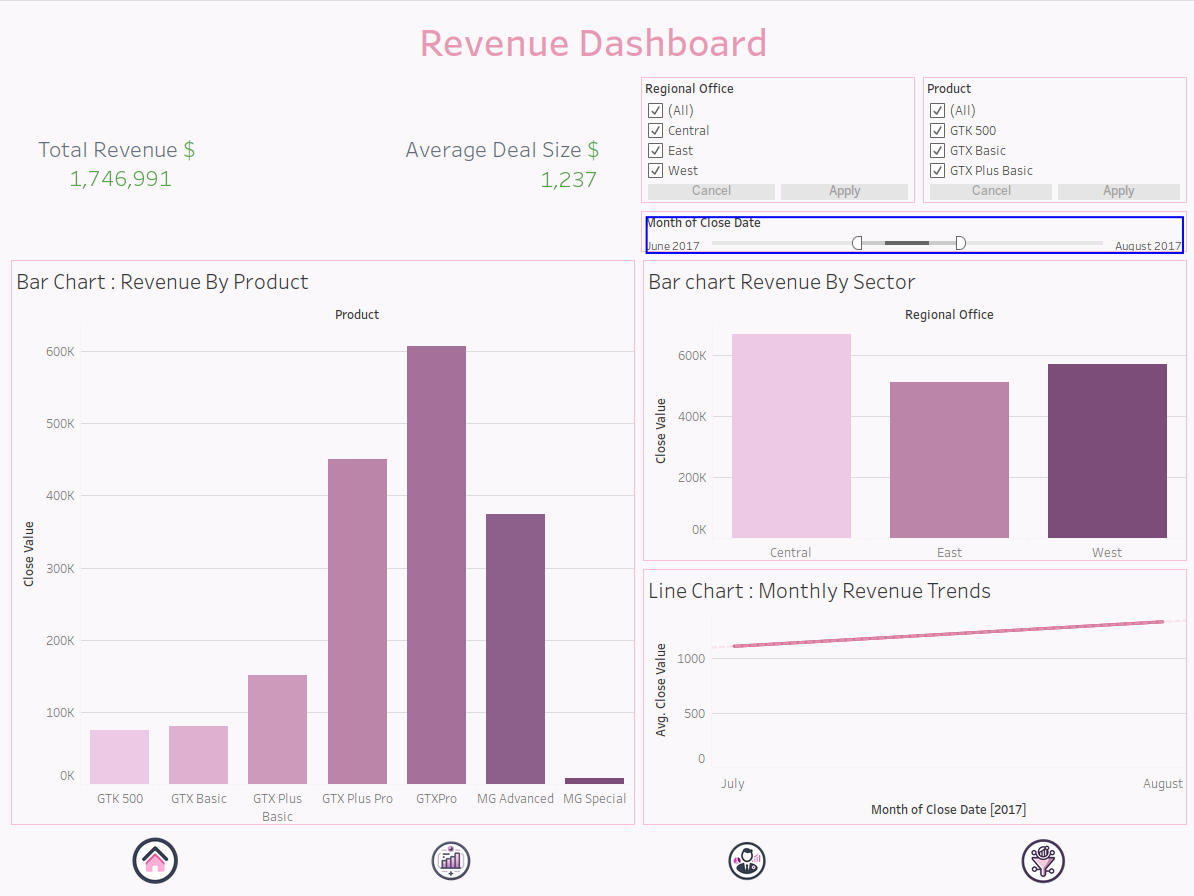
\includegraphics[width=0.8\textwidth]{resources/swappy-20240527_152550.png}
    \caption{Date Range Filter}
    \label{fig:date_range_filter}
\end{figure}

\clearpage
\section{Product Performance Dashboard}
% Product Performance Dashboard content goes here.
\begin{figure}[h!]
    \centering
    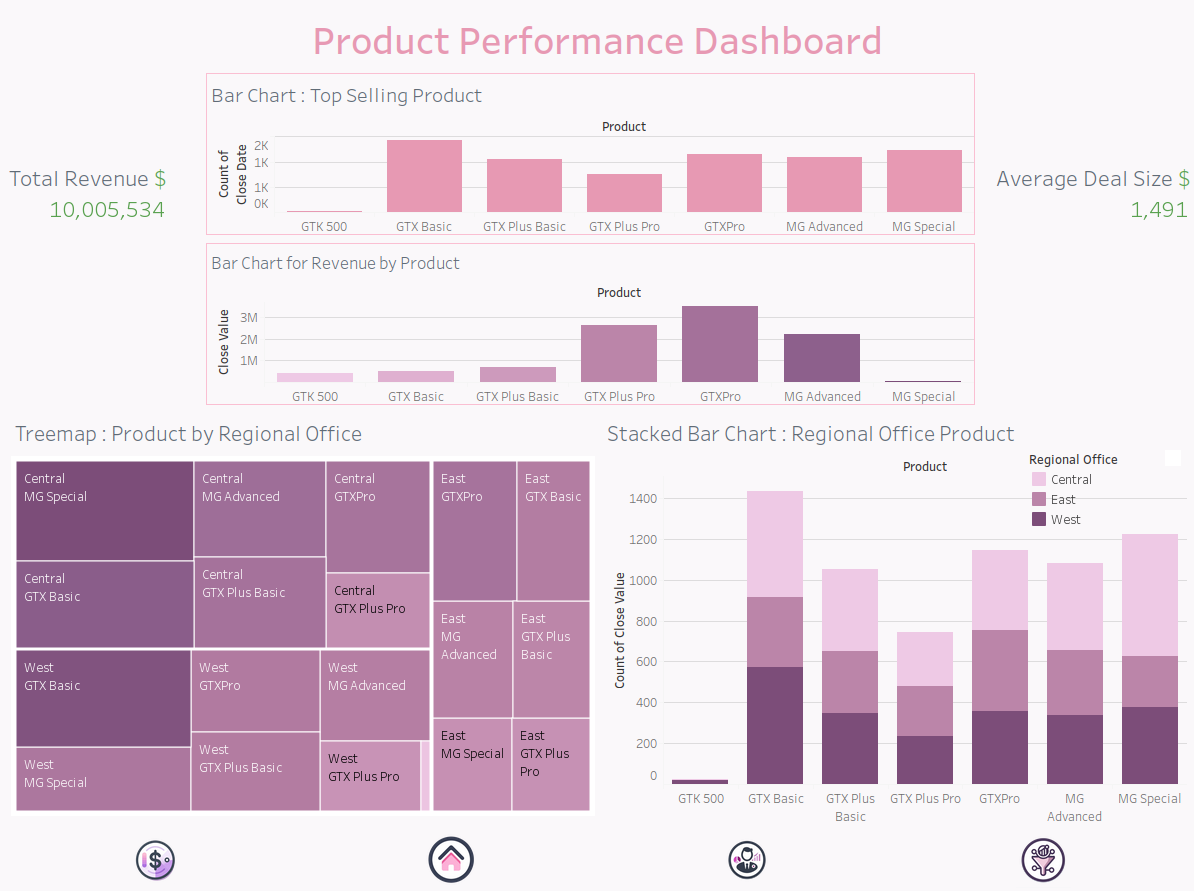
\includegraphics[width=0.8\textwidth]{resources/swappy-20240527_160325.png}
    \caption{Overview of the Product Performance Dashboard}
    \label{fig:product_performance_dashboard_overview}
\end{figure}
The Product Performance Dashboard provides detailed insights into the sales performance of different products. It includes key metrics and visualizations that help in understanding which products are performing well and their distribution across various regions.

\subsection{Key Metrics}
The key metrics displayed in the Product Performance Dashboard are:
\begin{itemize}
    \item \textbf{Total Revenue:} This metric shows the total revenue generated by all products over a specified period.
    \item \textbf{Average Deal Size:} This metric indicates the average revenue per deal for each product.
\end{itemize}

\subsection{Visualizations}
The Product Performance Dashboard includes the following visualizations:
\begin{itemize}
    \item \textbf{Bar Chart for Top Selling Product:} This bar chart displays the count of closed deals for each product.
    \item \textbf{Bar Chart for Revenue by Product:} This bar chart shows the revenue generated by each product.
    \item \textbf{Treemap for Product by Regional Office:} This treemap displays the distribution of product sales across different regional offices.
    \item \textbf{Stacked Bar Chart for Regional Office Product:} This stacked bar chart shows the count of closed deals for each product across different regional offices.
\end{itemize}


\subsection{Interactive Navigation}
Both the bar charts and the treemap can act as filters for the entire Product Performance Dashboard. Users can click on a specific bar or segment to filter the data across all visualizations on the dashboard, allowing for a more interactive and detailed analysis. There is also a {Regional Office Filter}.

\begin{figure}[h!]
    \centering
    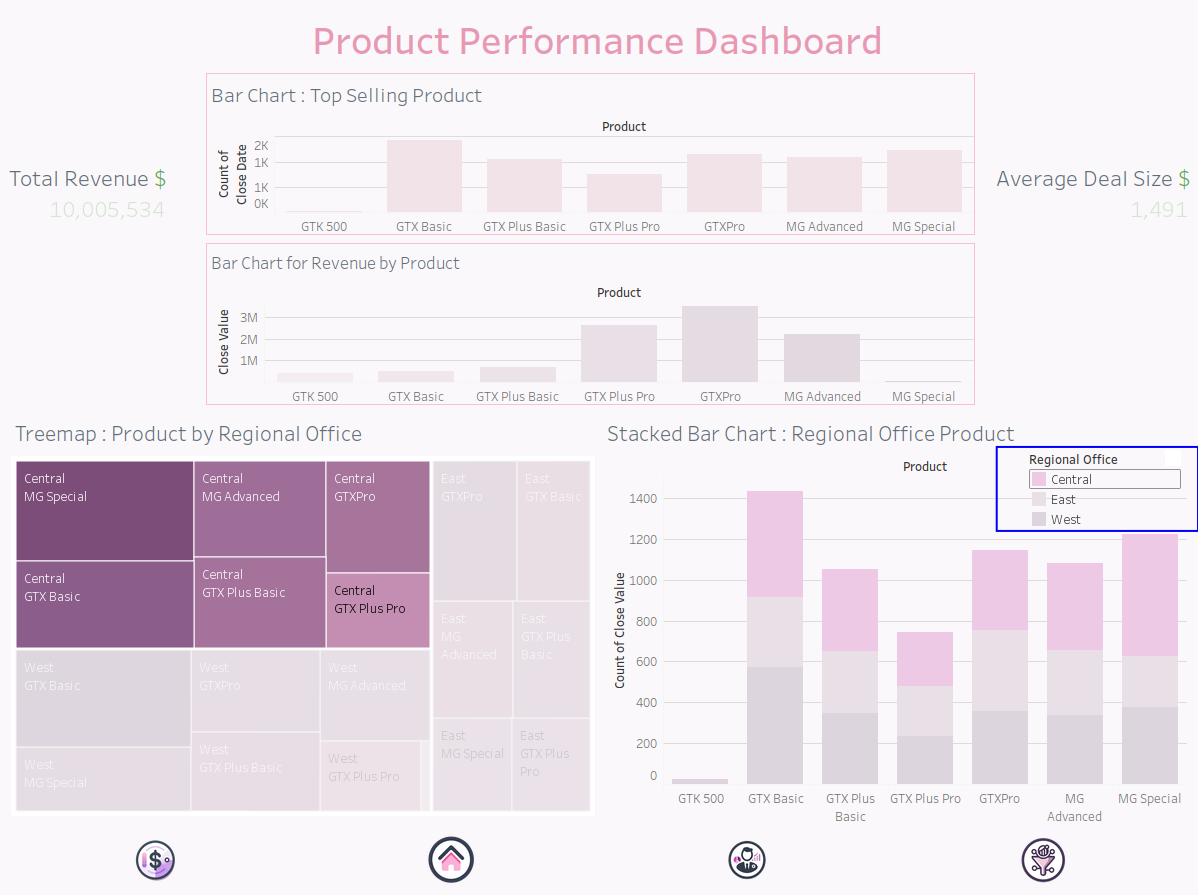
\includegraphics[width=0.8\textwidth]{resources/swappy-20240527_160008.png}
    \caption{Bar Chart for Top Selling Product}
    \label{fig:top_selling_product_bar_chart}
\end{figure}

\begin{figure}[h!]
    \centering
    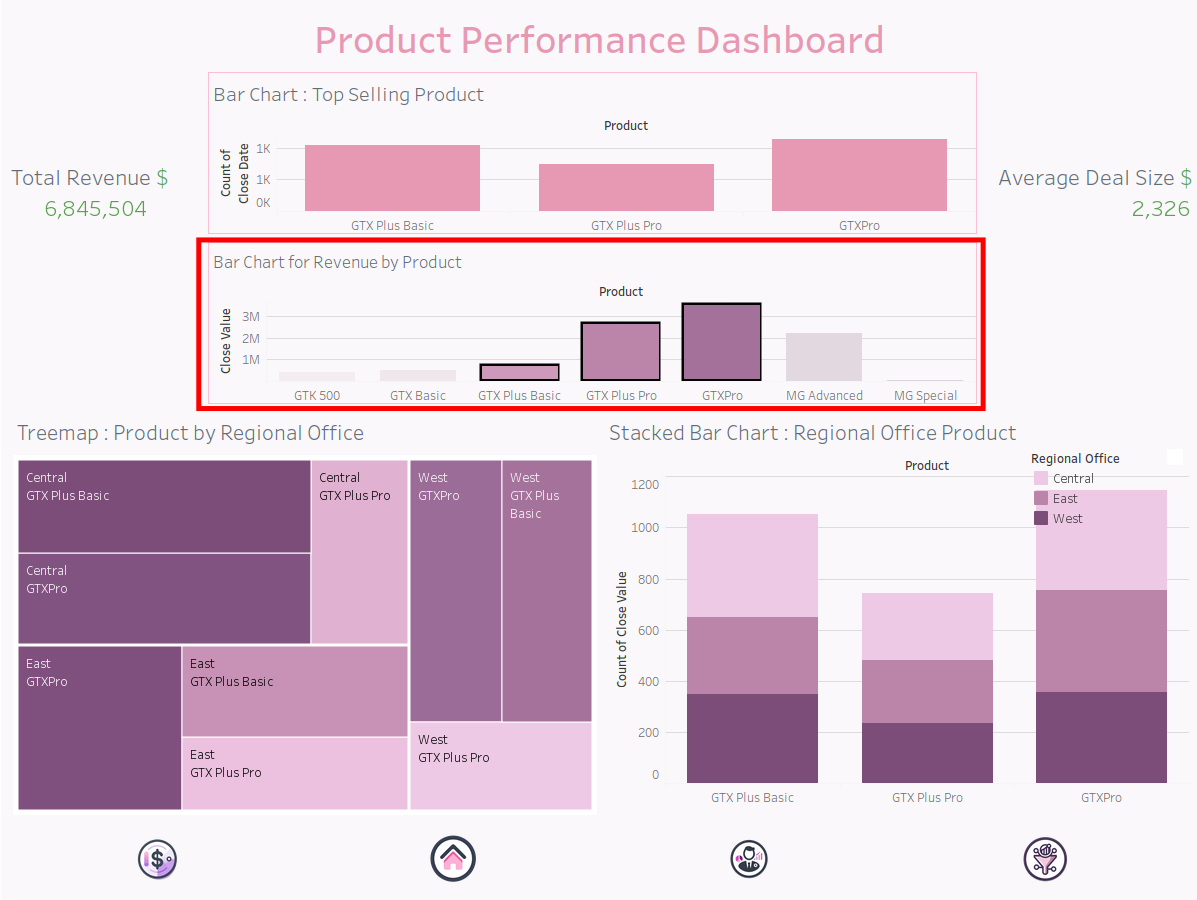
\includegraphics[width=0.8\textwidth]{resources/swappy-20240527_160042.png}
    \caption{Bar Chart for Revenue by Product}
    \label{fig:revenue_by_product_bar_chart}
\end{figure}

\begin{figure}[h!]
    \centering
    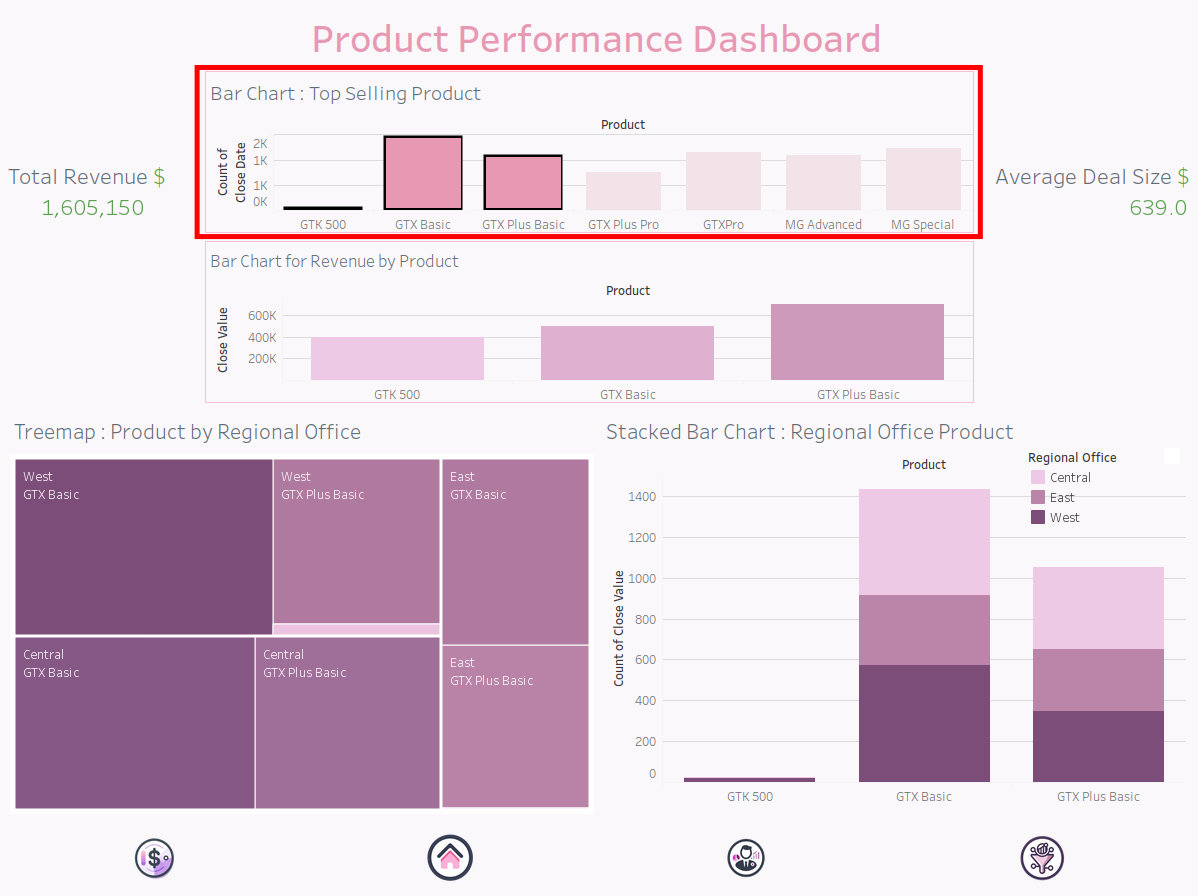
\includegraphics[width=0.8\textwidth]{resources/swappy-20240527_160111.png}
    \caption{Treemap for Product by Regional Office}
    \label{fig:product_by_regional_office_treemap}
\end{figure}
\clearpage

\section{Sales Team Dashboard}
% Sales Team Dashboard content goes here.
\begin{figure}[h!]
    \centering
    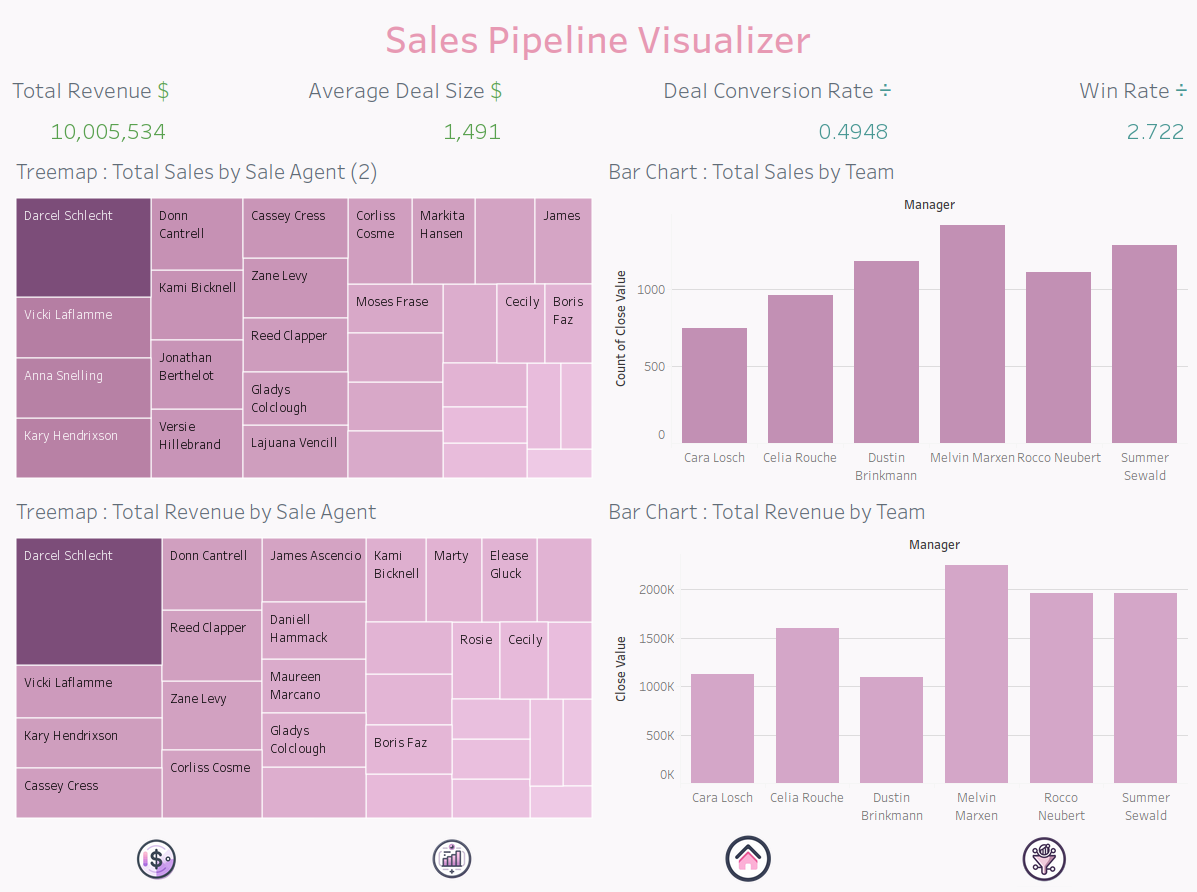
\includegraphics[width=0.8\textwidth]{resources/swappy-20240527_160845.png}
    \caption{Overview of the Sales Team Dashboard}
    \label{fig:sales_team_dashboard_overview}
\end{figure}

The Sales Team Dashboard provides detailed insights into the performance of individual sales agents and teams. It includes key metrics and visualizations that help in understanding the contribution of each sales agent and team to the overall sales performance.

\subsection{Key Metrics}
The key metrics displayed in the Sales Team Dashboard are:
\begin{itemize}
    \item \textbf{Total Revenue:} This metric shows the total revenue generated by the sales team over a specified period.
    \item \textbf{Average Deal Size:} This metric indicates the average revenue per deal for each sales agent.
    \item \textbf{Deal Conversion Rate:} This metric represents the percentage of deals that were successfully closed by the sales team.
    \item \textbf{Win Rate:} This metric shows the percentage of deals won out of the total deals engaged by the sales team.
\end{itemize}

\subsection{Visualizations}
The Sales Team Dashboard includes the following visualizations:
\begin{itemize}
    \item \textbf{Treemap for Total Sales by Sales Agent:} This treemap displays the total sales achieved by each sales agent.
    \item \textbf{Treemap for Total Revenue by Sales Agent:} This treemap shows the total revenue generated by each sales agent.
    \item \textbf{Bar Chart for Total Sales by Team:} This bar chart displays the count of closed deals for each sales team.
    \item \textbf{Bar Chart for Total Revenue by Team:} This bar chart shows the revenue generated by each sales team.
\end{itemize}

\subsection{Interactive Navigation}
Both the treemaps and the bar charts can act as filters for the entire Sales Team Dashboard. Users can click on a specific segment of the treemap or bar to filter the data across all visualizations on the dashboard, allowing for a more interactive and detailed analysis. There are also filters for different teams and managers.

\begin{figure}[h!]
    \centering
    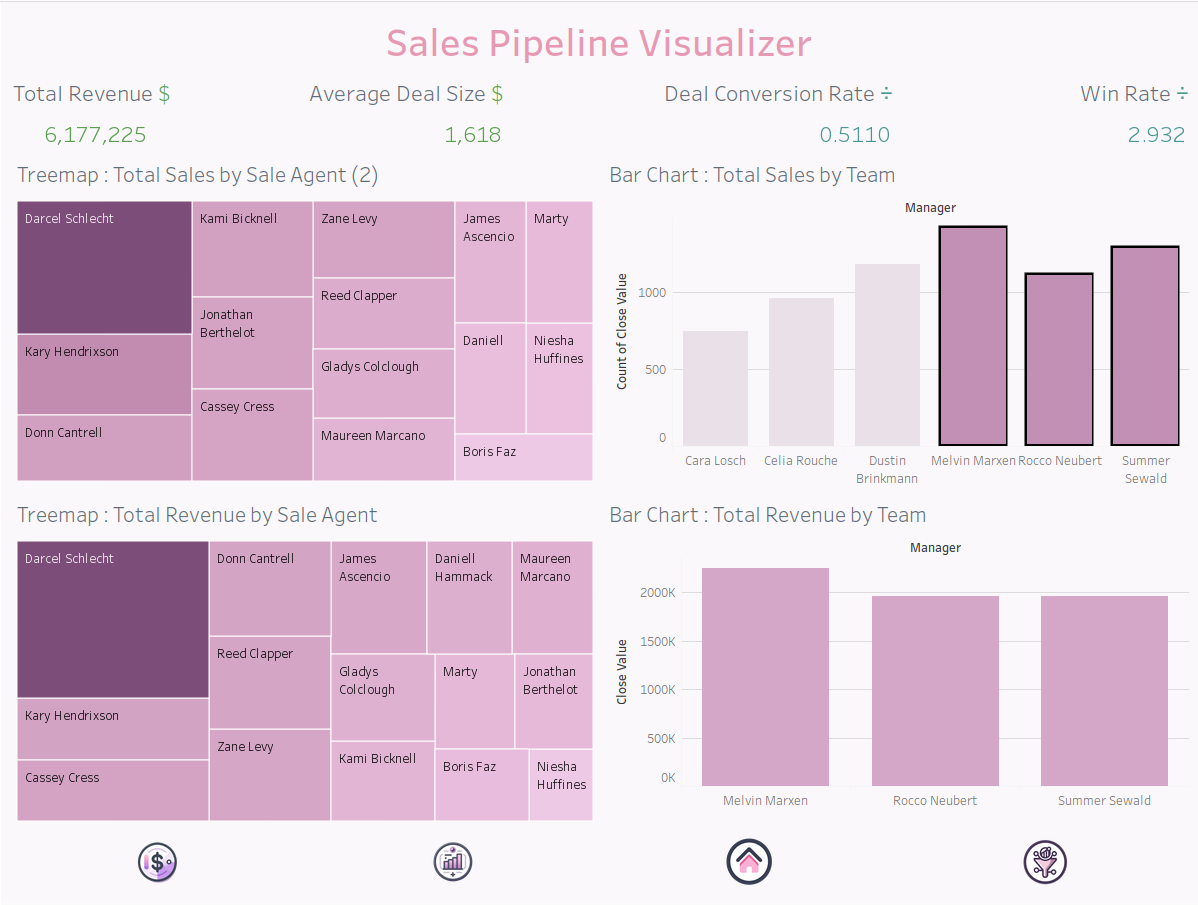
\includegraphics[width=0.8\textwidth]{resources/swappy-20240527_160904.png}
    \caption{Treemap applying a filter on sales agent performance.}
    \label{fig:sales_agent_treemap_filter}
\end{figure}

\begin{figure}[h!]
    \centering
    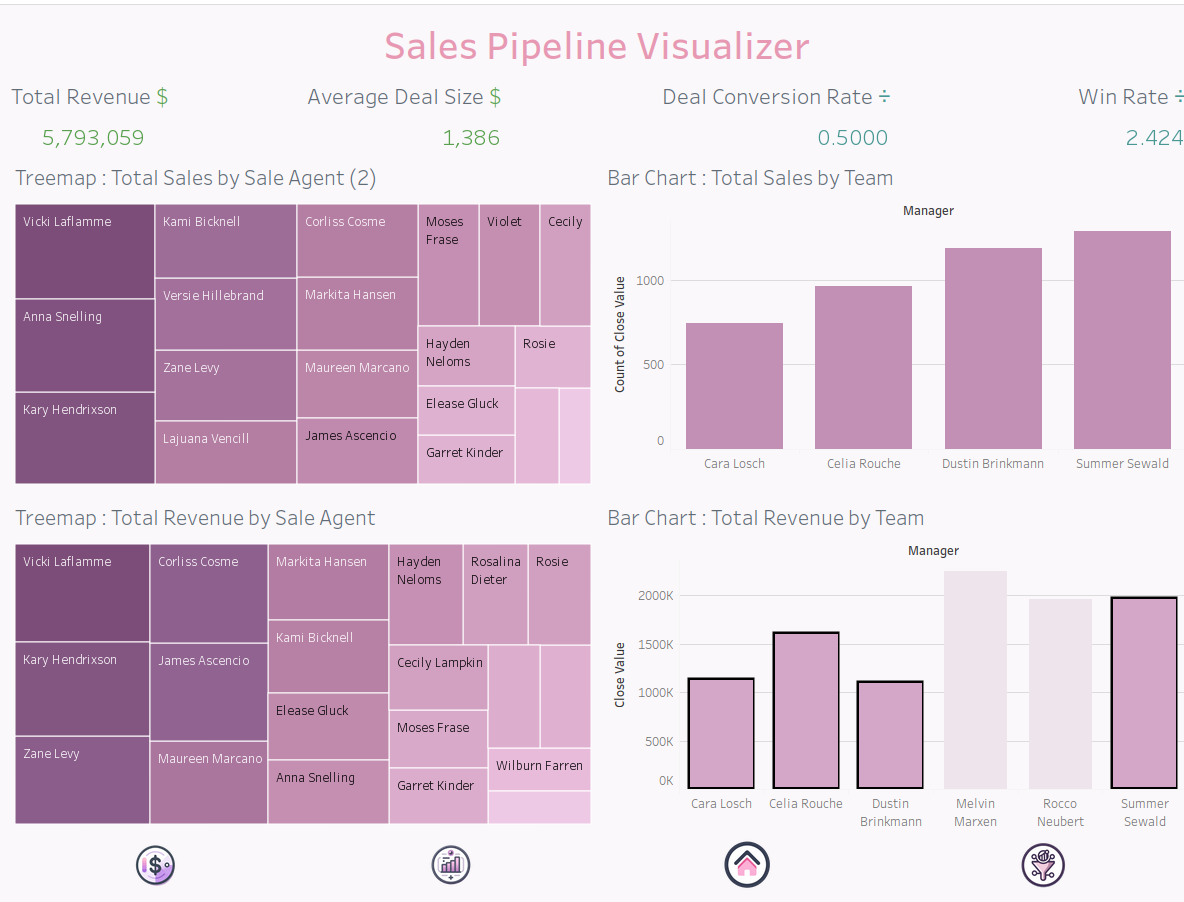
\includegraphics[width=0.8\textwidth]{resources/swappy-20240527_160924.png}
    \caption{Bar Chart applying a filter on team performance.}
    \label{fig:team_performance_bar_chart_filter}
\end{figure}

\clearpage

\section{Pipeline Analysis Dashboard}
% Pipeline Analysis Dashboard content goes here.
\begin{figure}[h!]
    \centering
    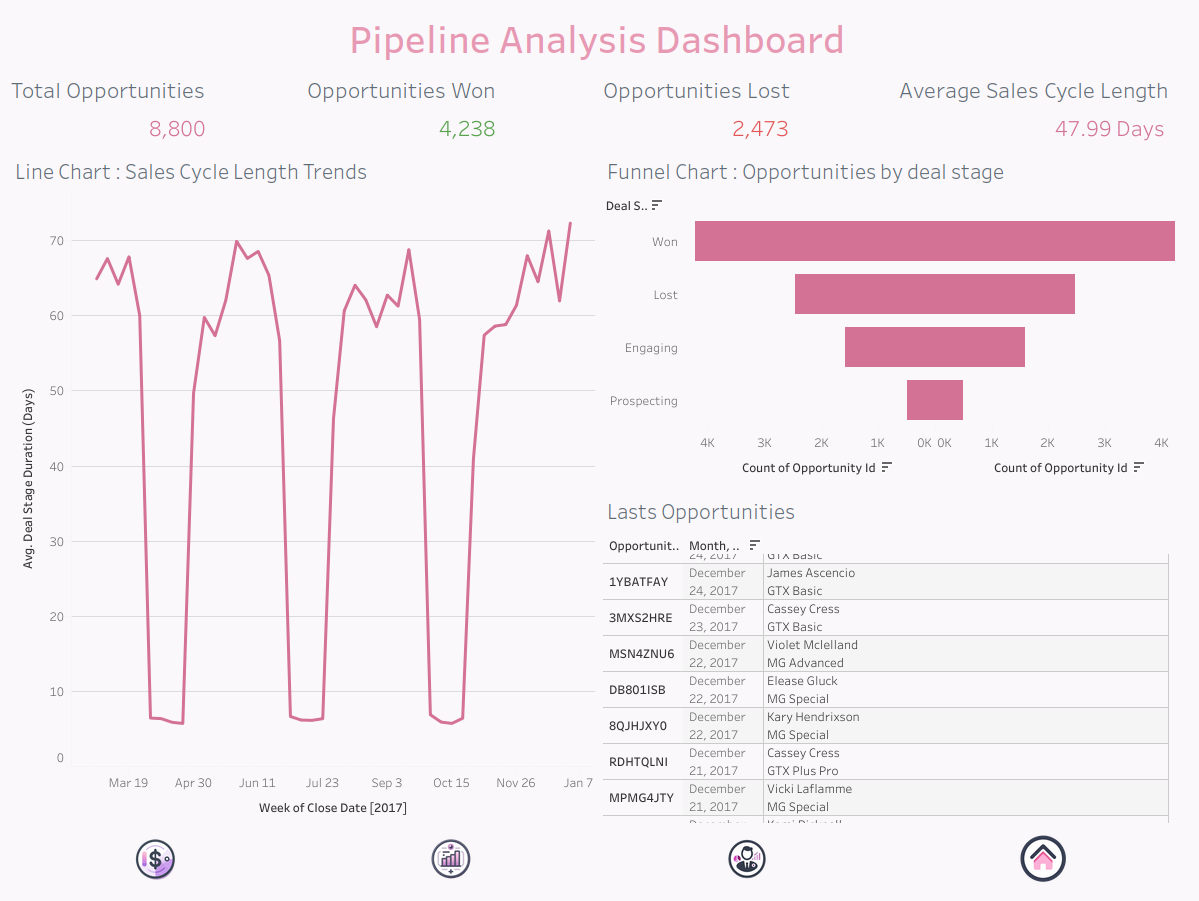
\includegraphics[width=0.8\textwidth]{resources/swappy-20240527_170251.png}
    \caption{Overview of the Pipeline Analysis Dashboard}
    \label{fig:pipeline_analysis_dashboard_overview}
\end{figure}
The Pipeline Analysis Dashboard provides detailed insights into the sales pipeline stages and performance. It includes key metrics and visualizations that help in understanding the opportunities at different stages of the sales cycle, trends in the sales cycle length, and recently closed opportunities.

\subsection{Key Metrics}
The key metrics displayed in the Pipeline Analysis Dashboard are:
\begin{itemize}
    \item \textbf{Total Opportunities:} This metric shows the total number of sales opportunities.
    \item \textbf{Opportunities Won:} This metric indicates the number of opportunities that were successfully closed.
    \item \textbf{Opportunities Lost:} This metric represents the number of opportunities that were not successfully closed.
    \item \textbf{Average Sales Cycle Length:} This metric shows the average duration of the sales cycle in days.
\end{itemize}

\subsection{Visualizations}
The Pipeline Analysis Dashboard includes the following visualizations:
\begin{itemize}
    \item \textbf{Line Chart for Sales Cycle Length Trends:} This line chart displays the average duration of the sales cycle over time.
    \item \textbf{Funnel Chart for Opportunities by Deal Stage:} This funnel chart shows the distribution of opportunities across different stages of the sales pipeline.
    \item \textbf{Table of Last Opportunities:} This table lists the most recent sales opportunities, including the opportunity ID, close date, sales agent, and product.
\end{itemize}

\end{document}
